\documentclass[11pt]{article}
\usepackage[a4paper,margin=24mm]{geometry}
\usepackage[T1]{fontenc}
\usepackage{lmodern,microtype,amsmath,amssymb,amsthm,mathtools,booktabs,longtable,array,graphicx}
\usepackage[hidelinks]{hyperref}
\hypersetup{pdftitle={Rare-event localization for adaptive threshold estimation},pdfauthor={AI-assisted research continuation},pdfsubject={Proved partial characterization, prior-art audit, and benchmark; v4 unchanged}}
\usepackage{enumitem,fancyhdr,needspace}
\setlength{\parskip}{4pt}
\setlength{\parindent}{0pt}
\setlist{nosep,leftmargin=1.4em}
\pagestyle{fancy}\fancyhf{}\fancyhead[L]{Adaptive threshold estimation: next-phase research}\fancyhead[R]{26 October 2026}\fancyfoot[C]{\thepage}
\setlength{\headheight}{14pt}
\newtheorem{theorem}{Theorem}[section]
\newtheorem{proposition}[theorem]{Proposition}
\newtheorem{lemma}[theorem]{Lemma}
\newtheorem{corollary}[theorem]{Corollary}
\theoremstyle{definition}\newtheorem{conjecture}[theorem]{Conjecture}
\newtheorem{definition}[theorem]{Definition}
\theoremstyle{remark}\newtheorem{remark}[theorem]{Remark}
\newcommand{\E}{\mathbb E}\newcommand{\PP}{\mathbb P}\newcommand{\R}{\mathbb R}
\newcommand{\ind}{\mathbf1}\newcommand{\kl}{\operatorname{kl}}\newcommand{\KL}{\operatorname{KL}}
\newcommand{\Var}{\operatorname{Var}}\newcommand{\TV}{\operatorname{TV}}
\newcommand{\Q}{\mathcal Q}\newcommand{\logp}{\log_+}
\newcommand{\status}[1]{\par\smallskip\noindent\textbf{Status: #1.}\par}
\title{Rare-event localization for adaptive threshold estimation\\[5pt]\large Proved partial characterization, prior-art audit, and a practical benchmark}
\author{AI-assisted research continuation\quad---\quad v4 preserved unchanged}
\date{26 October 2026}
\begin{document}
\maketitle
\begin{abstract}
We study the class of unknown sign functions $q$ with $\int q\,d\mu\le\rho$ at a fixed magnitude law $\mu$. The proposed rescaling $\rho\omega_\mu((\rho B)^{-1/2})$ is false for this global-rarity class: an explicit two-scale example separates it from the minimax error by an unbounded factor. We prove matching expected-budget root-mean-square and high-confidence rates for power margins $F(t)=(t/a)^\alpha$, $0<\alpha<2$, using a rare-region lower bound and a shifted-start version of the v4 classifier. For arbitrary laws, a variational functional $\Psi_{\mu,\rho}$ gives an all-adaptive lower bound by combining Lee--Valiant's single-coin information inequality with a bounded-likelihood-ratio decomposition. Its exact optimizer is controlled by a clipped inverse-square moment. A matching upper bound for every law is a conjecture, not a theorem in this note. A targeted primary-source audit records verified overlaps and unresolved priority questions. On Giles--Haji-Ali's model problem, independently tuned and held-out experiments favor their adaptive method over both the proved v4 reference and tuned variants. The comparison requires a model-specific Bernoulli conversion for v4 and reports its information loss, offline training expense, and sampling uncertainty. No novelty or publication-priority claim is made.
\end{abstract}

\textbf{Baseline integrity.} This is a separate continuation, not a rewrite or replacement of v4~\cite{baseline}. The package preserves the original PDF/source and records SHA-256 checks of the original PDF and ZIP.

\begin{center}\begin{tabular}{p{.58\textwidth}p{.31\textwidth}}\toprule
Claim or deliverable & Evidence status\\\midrule
Failure of the proposed rare-event rescaling & Proved; explicit counterexample\\
Matching power-margin rates, $0<\alpha<2$ & Proved; full arguments below\\
Arbitrary-law functional and lower bound & Proved; uses cited Lee--Valiant input\\
Arbitrary-law matching upper bound & Conjecture; not established\\
Practical performance comparisons & Numerical evidence only\\
Novelty and priority & Not certified; audit limits recorded\\\bottomrule
\end{tabular}\end{center}

\newpage
\tableofcontents
\newpage
\section{Experiment, localization, and the two anchors}
\status{Definitions and scope}
A fresh coin has $D\sim\mu$ on $(0,1/2]$, $S\mid D=d\sim\operatorname{Ber}(q(d))$, and probability
\[
 P=\tfrac12+(2S-1)D.
\]
Conditional on its latent probability, successive observations of that coin are independent Bernoulli trials. Distinct fresh coins are independent. An algorithm can create coins, revisit them, interleave their observations, and stop adaptively. It observes neither $D$ nor $S$. One observation is one unit of work. Arithmetic and independent randomization are not charged, as in v4.

Fix $0<\rho\le1/4$ and define
\begin{equation}\label{eq:class}
 \Q_\rho(\mu)=\left\{q:(0,1/2]\to[0,1]\text{ measurable}:\quad
 \theta(q):=\int q\,d\mu\le\rho\right\}.
\end{equation}
The quantity to estimate is $\theta(q)$, not the known upper bound $\rho$. Replacing the inequality by the known equality $\theta=\rho$ would trivialize estimation.

Let $R_{\mu,\rho}(B)$ be the infimum, over algorithms with $\sup_{q\in\Q_\rho}\E_qT\le B$, of $\sup_q(\E_q|\widehat\theta-\theta(q)|^2)^{1/2}$. Let $r_{\mu,\rho}(B,\delta)$ be the corresponding smallest uniform error radius at failure probability at most $\delta$. Here $B\ge1$ and $0<\delta\le1/4$. These are \emph{expected-work} criteria. The minimax benchmark may know $\mu,\rho$. Each construction's actual parameter requirements are stated separately.

This class deliberately permits the positives to concentrate in a difficult subpopulation. It does \emph{not} impose the stronger condition $q(d)\le\rho$ at every magnitude. Nor does it assume known conditional magnitude laws $\mu_+,\mu_-$. In the latter model the mixture weight is the main unknown; in \eqref{eq:class}, changing $q$ changes both conditional laws. Lee--Valiant's Section 7 addresses the known-conditional-law experiment with a per-coin depth restriction~\cite{lv}.

\subsection{Sanity checks}
For $\mu=\delta_\Delta$, the problem is the fixed-gap mixture experiment. The Lee--Valiant bounds~\cite{lv}, localized to $\theta\le\rho$, give, in the nontrivial regime $\varepsilon\le c\rho$,
\begin{equation}\label{eq:lvanchor}
 B^*(\varepsilon,\delta)\asymp
 \frac{\rho}{\varepsilon^2\Delta^2}\log(1/\delta).
\end{equation}
The corresponding error scale, saturated at the trivial radius, is
\[\min\{\rho,\sqrt{\rho\log(1/\delta)/B}/\Delta\}.\]
At fixed confidence or for RMS, omit the logarithmic factor. This is a cited anchor, not a new fixed-gap theorem.

For constant $\rho$, a correct localized scale must agree, up to constants, with v4's
\[
 \omega_\mu(h)=\E_\mu\min\{1,h/D\},\qquad h=B^{-1/2}
\]
(and $h=\sqrt{\log(1/\delta)/B}$ for high confidence). The proposed heuristic
\begin{equation}\label{eq:heuristic}
 H_{\mu,\rho}(h)=\rho\,\omega_\mu(h/\sqrt\rho)
\end{equation}
satisfies both anchors. The next section shows that this is insufficient.

\Needspace{8\baselineskip}
\section{A counterexample to the proposed rescaling}
\status{Proved; no numerical premise}
\begin{theorem}\label{thm:counter}
Let $0<\rho\le1/4$, $a=1/4$, $d=\rho^2$,
\[
 \mu_\rho=\rho\delta_d+(1-\rho)\delta_a,\qquad B=\rho^{-4}.
\]
Then $R_{\mu_\rho,\rho}(B)\ge\rho/100$, whereas
\[
 H_{\mu_\rho,\rho}(B^{-1/2})
 =\rho^2+4(1-\rho)\rho^{5/2}=O(\rho^2).
\]
The minimax error is therefore of order $\rho$, and the heuristic can underestimate it by an unbounded factor.
\end{theorem}
\begin{proof}
Put $\eta=1/64$ and choose $q_\pm(d)=1/2\pm\eta$, $q_\pm(a)=0$. Both targets lie in $[0,\rho]$ and are separated by $\Delta=2\eta\rho=\rho/32$. Even if the algorithm is told every magnitude, only a queried coin of magnitude $d$ is informative. The v4 posterior inequality gives, for every next observation and every history,
\[
 \KL_{\rm next}\le\frac{32d^2\eta^2}{(1-4\eta^2)^2}.
\]
The stopped chain rule and $Bd^2=1$ imply $\KL(\mathsf P_+,\mathsf P_-)\le k_0:=32\eta^2/(1-4\eta^2)^2<0.008$. Hence $\TV\le\sqrt{k_0/2}$. Thresholding an estimator halfway between the two targets gives error sum at most $8R^2/\Delta^2$, whereas every test has error sum at least $1-\TV$. Thus
\[
 R\ge\Delta\sqrt{(1-\sqrt{k_0/2})/8}>\rho/100.
\]
The constant estimator $\rho/2$ has error at most $\rho/2$. Finally, $(\rho B)^{-1/2}=\rho^{3/2}$ lies between $d$ and $a$. Direct substitution in \eqref{eq:heuristic} gives the stated expression.
\end{proof}

The hard subpopulation contains both positive and negative near-threshold coins. Its local positive fraction is close to $1/2$, although its total population mass is only $\rho$. Multiplying the global modulus by $\rho$ incorrectly treats the difficult portion as if positives were thinly spread across all magnitudes. Section~\ref{sec:power} also gives a failure example with one fixed, uniform magnitude law, so this is not merely an artifact of changing $\mu$ with $\rho$.

\section{Two localized lower bounds for arbitrary laws}
\subsection{A balanced-region bound independent of rare-prior machinery}
\status{Proved from the v4 information inequality}
Define
\begin{equation}\label{eq:Gamma}
 \Gamma_{\mu,\rho}(h)=
 \sup_{A:\,\mu(A)\le\rho}\int_A\min\{1,h/d\}\,\mu(dd).
\end{equation}
\begin{proposition}\label{prop:Gamma}
There is a universal $c>0$ such that
\[
 R_{\mu,\rho}(B)\ge c\Gamma_{\mu,\rho}(B^{-1/2}),\qquad
 r_{\mu,\rho}(B,\delta)\ge c\Gamma_{\mu,\rho}\left(\sqrt{\log(1/\delta)/B}\right).
\]
This lower bound remains valid with revealed or selected magnitudes.
\end{proposition}
\begin{proof}
For any admissible $A$, put
$q_\pm(d)=\ind_A(d)[1/2\pm\eta_h(d)]$ with
$\eta_h(d)=\frac18\min(1,h/d)$. The larger target is at most $5\mu(A)/8\le\rho$. The target separation is
$\Delta_h=\frac14\int_A\min(1,h/d)\,d\mu$.
Every observation has predictive KL at most $128h^2/225$ by v4, and observations outside $A$ have zero divergence. Thus transcript KL is at most $128Bh^2/225$.
For RMS choose $h=c_0B^{-1/2}$ with a sufficiently small universal $c_0$ and use the testing argument above. For confidence use $h=c_1\sqrt{\log(1/\delta)/B}$, choosing $c_1$ so that transcript KL is strictly less than $\kl(1-\delta,\delta)$; an estimator with radius smaller than $\Delta_h/2$ would contradict data processing. The integrand satisfies $\min(1,\lambda h/d)\ge\lambda\min(1,h/d)$ for $0<\lambda\le1$. Taking the supremum over $A$ proves the claims without changing the scale.
\end{proof}

Atoms can prevent $\Gamma$ from using a small amount of mass at a magnitude. The next functional permits fractional allocation and includes the fixed-gap rarity factor.

\subsection{A variational lower modulus}
\status{Proved lower bound; matching general upper bound not proved}
Define
\begin{equation}\label{eq:Psi}
 \Psi_{\mu,\rho}(h)=
 \sup_{\substack{0\le w\le1\\\int w\,d\mu\le\rho}}
 \int\min\{w(d),\,h\sqrt{w(d)}/d\}\,\mu(dd).
\end{equation}
The optimization variable $w$ represents how a hard alternative allocates its available positive mass. It is not an assumed or estimated sign function of the true population.

\begin{lemma}[Published single-coin input]\label{lem:LV}
There are universal constants $c_*,C_*>0$ such that, for $0<u\le c_*$, $0\le v\le c_*u$, $0<d\le1/2$, and any stopped single-coin adaptive experiment, its transcript laws under sign priors $u$ and $u+v$ satisfy
\begin{equation}\label{eq:single}
 H^2(\mathsf P_u,\mathsf P_{u+v})\le
 C_*\frac{v^2d^2}{u}\E_u\tau.
\end{equation}
Here $H^2(P,Q)=1-\int\sqrt{dP\,dQ}$ and external, parameter-independent randomization is allowed.
\end{lemma}
\begin{proof}[Source and extension]
For sufficiently small $d$, this is the first expected-work bound in Lee--Valiant Corollary 19~\cite{lv}, with their $\rho,\epsilon,\Delta$ replaced by $u,v,d$. Their result averages over histories and is not a history-uniform predictive-KL claim. Its proof is not reproduced here; it is an explicit external theorem used by this note.
For $d\ge d_*>0$, reveal the sign at the first requested observation. Before that request the experiment has no sign information. By data processing, the Hellinger distance is at most the probability of making the first request times the distance between $\operatorname{Ber}(u)$ and $\operatorname{Ber}(u+v)$. The latter is at most $C v^2/u$ when $u$ and $v/u$ are small. Since $\E_u\tau$ is at least that request probability and $d^2\ge d_*^2$, this proves \eqref{eq:single} on the remaining range, including deterministic coins at $d=1/2$. Increasing a universal constant joins the two ranges.
\end{proof}

\begin{lemma}[Bounded-ratio decomposition]\label{lem:hybrid}
Consider two independent-coin population laws $\nu_0,\nu_1$ whose latent Radon--Nikodym ratio lies in $[1-\kappa,1+\kappa]$ for some fixed $\kappa<1$. For a fully adaptive experiment stopped after at most $n$ observations, let $P_0,P_1$ be its transcript laws. Let $P_i$ be the hybrid law using $\nu_1$ only for coin $i$ and $\nu_0$ for every other coin. Then
\[
 \KL(P_0,P_1)\le C_\kappa\sum_i H^2(P_0,P_i).
\]
The same conclusion holds by finite-prefix limits for almost-surely terminating experiments whenever the right-hand side is uniformly bounded along the prefixes.
\end{lemma}
\begin{proof}
Index coins in order of their first observation, so at most $n$ indices occur. Include the algorithm's independent random seed in the transcript. For a fixed transcript, let $L_i=dP_i/dP_0$. This is the local coin likelihood ratio, marginalized over that coin's latent state, so $1-\kappa\le L_i\le1+\kappa$. Independence of latent coins and the parameter-independent action rule give
\[
 \frac{dP_1}{dP_0}=\prod_iL_i.
\]
This identity holds even though the local sequence lengths were chosen using other coins' outcomes. Also $\E_0L_i=1$. On this compact ratio interval,
$-\log x+(x-1)\le C_\kappa(x-1)^2$, and
$(x-1)^2\le C_\kappa(\sqrt x-1)^2$. Taking expectations and using
$\E_0(\sqrt{L_i}-1)^2=2H^2(P_0,P_i)$ proves the finite-prefix claim. Increasing stopped-transcript sigma fields and the standard monotone limit of relative entropy prove the last assertion. Applying the argument at finite prefixes avoids any unjustified interchange of an unbounded stopping sum and a likelihood derivative.
\end{proof}

This lemma is the bounded-relative-change mechanism of Lee--Valiant Lemma 18, stated for the present magnitude-dependent perturbations. It is not a new general decomposition principle. Unlike an attempted uniform posterior bound, it charges informative but rare histories by their expected frequency.

\begin{theorem}[Arbitrary-law rare-event lower bound]\label{thm:PsiLower}
For the ordinary iid fresh-coin experiment, there is a universal $c>0$ such that
\begin{align}
 R_{\mu,\rho}(B)&\ge c\Psi_{\mu,\rho}(B^{-1/2}),\label{eq:psilowr}\\
 r_{\mu,\rho}(B,\delta)&\ge c\Psi_{\mu,\rho}\left(\sqrt{\log(1/\delta)/B}\right).\label{eq:psilowh}
\end{align}
The proof uses Lemma~\ref{lem:LV}; it does not assert this strengthened bound for an arbitrary selected-magnitude oracle.
\end{theorem}
\begin{proof}
Fix any feasible $w$ in \eqref{eq:Psi} and write $f_h(d)=\min\{w(d),h\sqrt{w(d)}/d\}$. Choose small universal constants $b>0$ and $c_0>0$ with $c_0\ll b$ and $b+c_0\le1$. Define
\[
 q_0(d)=bw(d),\qquad q_1(d)=bw(d)+c_0f_h(d).
\]
Both belong to \eqref{eq:class}. Their target separation is $c_0\int f_h\,d\mu$.
Where $w>0$, put $u=bw$, $v=c_0f_h$. The relative change $v/u$ is uniformly small and
\begin{equation}\label{eq:localcost}
 \frac{v^2d^2}{u}\le \frac{c_0^2}{b}h^2.
\end{equation}
Where $w=0$ the two laws agree. The sign-prior likelihood ratios, and hence the latent coin ratios, are uniformly in $[1-\kappa,1+\kappa]$ for a fixed $\kappa<1$.

At a finite observation prefix, apply Lemma~\ref{lem:hybrid}. To bound its $i$th term, simulate all other coins under $q_0$ as external randomness, and reveal $D_i$ only for the purpose of bounding information. Conditional on $D_i=d$, this is a single-coin stopped experiment with priors $u(d),u(d)+v(d)$. Data processing, Lemma~\ref{lem:LV}, and \eqref{eq:localcost} give
\[
 H^2(P_0,P_i)\le C h^2\E_0\tau_i.
\]
Here the conditional distributions of all simulated coins and the algorithmic seed are the same in both worlds. Summing over coins counts each observation once. Thus
\[
 \KL(P_0,P_1)\le C h^2\E_0(T\wedge n)\le Ch^2B.
\]
Let $n$ tend to infinity. For RMS choose a small constant multiple of $B^{-1/2}$; for confidence choose a small constant multiple of $\sqrt{\log(1/\delta)/B}$. The same two-point testing arguments as Proposition~\ref{prop:Gamma} apply. Finally, $\Psi(\lambda h)\ge\lambda\Psi(h)$ for $0<\lambda\le1$, and taking the supremum over $w$ yields the stated scales.
\end{proof}

\subsection{An exact solution of the variational problem}
\status{Proved functional identity; not a general minimax upper theorem}
\begin{proposition}\label{prop:optimizer}
For $0<\rho<1$, let $t=t_{\mu,\rho}>0$ be the unique solution of
\begin{equation}\label{eq:tcut}
 \E_\mu\min\{1,t^2/D^2\}=\rho.
\end{equation}
Then $w_*(d)=\min\{1,t^2/d^2\}$ is an optimizer in \eqref{eq:Psi} for every $h>0$. If $h\ge t$, then $\Psi_{\mu,\rho}(h)=\rho$. If $0<h<t$, then
\begin{equation}\label{eq:psiform}
 \Psi_{\mu,\rho}(h)=F_\mu(h)
 +h\E_\mu[D^{-1};\,h<D\le t]
 +ht\E_\mu[D^{-2};\,D>t].
\end{equation}
These identities allow atoms and singular laws.
\end{proposition}
\begin{proof}
The left side of \eqref{eq:tcut} is continuous, tends to zero at $t=0$, and is strictly increasing until it reaches one. This proves existence and uniqueness at $\rho<1$.
For $h<t$, put $\lambda=h/(2t)<1/2$. For fixed $d$, the concave function
$f_d(w)=\min\{w,(h/d)\sqrt w\}$ is linear until $w=(h/d)^2$, then square-root, on $[0,1]$. Maximizing $f_d(w)-\lambda w$ on $[0,1]$ gives exactly $w_*(d)$: in the square-root portion its stationary point is $t^2/d^2$, and otherwise the maximum is at $1$. Integration and $\int w_*\,d\mu=\rho$ prove optimality. Splitting at $h$ and $t$ gives \eqref{eq:psiform}, with the endpoint contributions agreeing if there are atoms. If $h\ge t$, $f_d(w_*)=w_*$ everywhere, so the objective equals the maximum possible value $\rho$.
\end{proof}

In particular,
\begin{equation}\label{eq:anchorspsi}
 \Psi_{\delta_\Delta,\rho}(h)=\min\{\rho,h\sqrt\rho/\Delta\},\qquad
 \rho\omega_\mu(h/\sqrt\rho)\le\Psi_{\mu,\rho}(h)\le\omega_\mu(h).
\end{equation}
The heuristic is the feasible \emph{constant allocation} $w\equiv\rho$ in the variational problem. Its failure is an allocation failure, not a failure of its two sanity anchors. If $\rho$ stays bounded away from zero, \eqref{eq:anchorspsi} recovers v4's modulus up to constants. The inverse-square tail in \eqref{eq:psiform} describes how hard negative coins outside the unresolved core still contribute.

\begin{conjecture}[Unresolved arbitrary-law upper bound]\label{conj:full}
For every magnitude law, with uniform constants,
\[
 R_{\mu,\rho}(B)\asymp\Psi_{\mu,\rho}(B^{-1/2}),\qquad
 r_{\mu,\rho}(B,\delta)\asymp
 \Psi_{\mu,\rho}\left(\sqrt{\log(1/\delta)/B}\right).
\]
Only the lower inequalities are established here in full generality. No distribution-blind algorithm attaining the upper inequalities for arbitrary $\mu$ is supplied.
\end{conjecture}

\section{Matching rare-event rates for power margins}\label{sec:power}
\status{Proved for $0<\alpha<2$; constants depend on $\alpha$}
Let $\mu_{\alpha,a}$ have $F(t)=(t/a)^\alpha$ on $(0,a]$, with $0<a\le1/4$. Write
\begin{equation}\label{eq:rscale}
 \mathcal R_{\alpha,\rho}(x)=
 \begin{cases}
 \min\{\rho,x^\alpha\},&0<\alpha<1,\\
 \min\{\rho,x[1+\logp(\rho/x)]\},&\alpha=1,\\
 \min\{\rho,\rho^{1-1/\alpha}x\},&1<\alpha<2.
 \end{cases}
\end{equation}
\begin{theorem}\label{thm:power}
For fixed $0<\alpha<2$, all $0<a\le1/4$, $0<\rho\le1/4$, $B\ge1$, and $0<\delta\le1/4$,
\begin{align*}
 R_{\mu_{\alpha,a},\rho}(B)&\asymp_\alpha
 \mathcal R_{\alpha,\rho}\bigl((a\sqrt B)^{-1}\bigr),\\
 r_{\mu_{\alpha,a},\rho}(B,\delta)&\asymp_\alpha
 \mathcal R_{\alpha,\rho}\bigl(a^{-1}\sqrt{\log(1/\delta)/B}\bigr).
\end{align*}
The same upper bounds hold for every magnitude law with $F_\mu(t)\le\min\{(t/a)^\alpha,1\}$. The upper construction knows $(\alpha,a,\rho)$, not the individual magnitudes or sign function. It is not the general distribution-blind rare-event algorithm posited in Conjecture~\ref{conj:full}.
\end{theorem}

\subsection{Lower proof}
Take $A=(0,a\rho^{1/\alpha}]$ in Proposition~\ref{prop:Gamma}. Its mass is $\rho$. Put $t_\rho=a\rho^{1/\alpha}$. For $h\ge t_\rho$ the restricted modulus is $\rho$. For $h<t_\rho$ it is
\begin{equation}\label{eq:restrictedpower}
 \left(\frac h a\right)^\alpha+
 \frac{\alpha h}{a^\alpha}\int_h^{t_\rho}d^{\alpha-2}\,dd.
\end{equation}
For $\alpha\ne1$, the integral is
$(t_\rho^{\alpha-1}-h^{\alpha-1})/(\alpha-1)$; for $\alpha=1$ the result is
$(h/a)[1+\log(a\rho/h)]$. These expressions are comparable, with constants depending only on $\alpha$, to \eqref{eq:rscale}. This proof uses the balanced rare-region construction and does not need the imported single-coin rare-prior lemma.

\subsection{Why v4's unmodified variance is not rarity-scaled}
\begin{proposition}\label{prop:noise}
Fix an interior magnitude $0<d<1/2$ and let every coin be negative. For v4's untruncated geometric single-term estimator $Y$, which is unbiased and square-integrable at this fixed gap,
\[
 \Var Y\ge\frac{1/2-d}{1-2^{-1/2}}>0.
\]
For the truncation at level $L$, the same second-moment lower bound holds, and
$\Var Y_L\ge(1/2-d)/(1-2^{-1/2})-(\E Z_{2^L})^2$.
\end{proposition}
\begin{proof}
The event $J=0$ has probability $p_0=1-2^{-1/2}$ and contributes $Y=X/p_0$ for one Bernoulli observation with success probability $1/2-d$. Therefore $\E Y^2\ge(1/2-d)/p_0$. In the untruncated case $\E Y=0$. In the truncated case telescoping gives $\E Y_L=\E Z_{2^L}$; subtract its square.
\end{proof}
This is an analytic obstruction to deriving a $\rho$ factor by reusing v4's second-moment estimate unchanged. At $d=1/4$ the lower floor is approximately $0.8536$, even though $\theta=0$.

\subsection{A shifted-start construction}
Retain v4's classifier $Z_n$ with dyadic checkpoints and threshold
$\sqrt{[1+\log(n/k)]/k}$ at checkpoint $k<n$. Define
\[
 e_n(d)=\min\{1,(nd^2)^{-2}\},\qquad
 m_n(d)=\min\{n,d^{-2}[1+\logp(nd^2)]\}.
\]
The v4 conditional inequalities are
$\PP(Z_n\ne S\mid d,S)\le e_n(d)$ and
$\E(\tau_n\mid d,S)\le17m_n(d)$~\cite{baseline}.

\begin{lemma}\label{lem:integrals}
For $na^2\ge1$ and $0<\alpha<2$,
\begin{align}
 e_n:=\E_{\mu_{\alpha,a}}e_n(D)&\le K_e a^{-\alpha}n^{-\alpha/2},&K_e&=\frac4{4-\alpha},\label{eq:eb}\\
 \E_{\mu_{\alpha,a}}m_n(D)&\le K_m a^{-\alpha}n^{1-\alpha/2},&
 K_m&=1+\frac\alpha{2-\alpha}+\frac{2\alpha}{(2-\alpha)^2}.\label{eq:mb}
\end{align}
The same bounds hold under the stated stochastic-dominance envelope.
\end{lemma}
\begin{proof}
Split each integral at $d=n^{-1/2}$. For \eqref{eq:eb}, the first part is $(a\sqrt n)^{-\alpha}$; extending the remaining power integral to infinity gives the factor $1+\alpha/(4-\alpha)$. For \eqref{eq:mb}, substitute $u=d\sqrt n$ in the tail and extend its upper endpoint to infinity. The remaining factor is
\[
 1+\alpha\int_1^\infty u^{\alpha-3}(1+2\log u)\,du
 =K_m.
\]
Both integrands are nonincreasing in $d$, which proves the envelope statement. The restriction $\alpha<2$ is essential to this particular work bound.
\end{proof}

Choose the smallest dyadic $n_0$ satisfying
\begin{equation}\label{eq:n0}
 n_0\ge a^{-2}(K_e/\rho)^{2/\alpha}.
\end{equation}
If $B<4n_0$, return $\rho/2$. Otherwise choose $N=n_02^L$ as the largest such number with $4N\le B$. Thus $B/8<N\le B/4$. Set $n_j=n_02^j$ and
\[
 \Delta_0=Z_{n_0},\qquad \Delta_j=Z_{n_j}-Z_{n_{j-1}},\quad j\ge1,
\]
using a shared observation prefix within each increment. Sample $J$ with
$p_j=(1-r)r^j$, $r=2^{-1/2}$, and return $Y_L=\Delta_J/p_J$ if $J\le L$ and zero otherwise. Coins are independent between calls. The observed work $C_L$ is at most $N$.

\begin{lemma}\label{lem:shiftbounds}
With $S_L=\sum_{j=0}^L n_j^{(1-\alpha)/2}$, uniformly over the rare-event envelope class,
\begin{align}
 |\E Y_L-\theta|&\le K_e a^{-\alpha}N^{-\alpha/2},\label{eq:shiftbias}\\
 \E Y_L^2&\le C_\alpha a^{-\alpha}n_0^{-1/2}S_L,\label{eq:shiftvar}\\
 \E C_L&\le C_\alpha a^{-\alpha}n_0^{1/2}S_L.\label{eq:shiftwork}
\end{align}
\end{lemma}
\begin{proof}
Telescoping proves \eqref{eq:shiftbias}. At the base,
$\E Z_{n_0}^2=\PP(Z_{n_0}=1)\le\theta+e_{n_0}\le2\rho$.
Dyadic rounding in \eqref{eq:n0} gives
$\rho\le2^{\alpha/2}K_e a^{-\alpha}n_0^{-\alpha/2}$, so the base obeys the same power envelope as the increments. For $j\ge1$,
\[
 \E\Delta_j^2\le e_{n_j}+e_{n_{j-1}}\le C_\alpha a^{-\alpha}n_j^{-\alpha/2}.
\]
Divide by $p_j=(1-r)\sqrt{n_0/n_j}$ and sum to obtain \eqref{eq:shiftvar}. For work, a coupled increment costs at most the sum of the two classifier costs, so its expectation is at most $34K_m a^{-\alpha}n_j^{1-\alpha/2}$; the base needs only the factor $17$. Multiply by $p_j$ and sum to obtain \eqref{eq:shiftwork}.
\end{proof}

\subsection{Calibration and completion of the upper proof}
Apply the exact v4 two-success wrapper to iid pairs $(Y_L,C_L)$, with cap $N$. Its pilot markers have success probability $C_L/N$. Stop at the second success, at pilot count $K$, discard the pilot values, and average $K-1$ fresh production values. With $c=\E C_L>0$ and $v=\Var Y_L$, the identities are
\begin{equation}\label{eq:calibration}
 \E T=4N-c\le B,\quad \E\widehat\theta=\E Y_L,\quad
 \Var\widehat\theta=vc/N.
\end{equation}
The identity $\E[1/(K-1)]=c/N$ is classical inverse-binomial estimation; the wrapper is inherited from v4, not claimed as new~\cite{baseline,mendo}. Independence of the fresh production samples is essential.

Equations \eqref{eq:shiftbias}--\eqref{eq:shiftwork} imply
\begin{equation}\label{eq:upperwork}
 \bigl(\E|\widehat\theta-\theta|^2\bigr)^{1/2}
 \le C_\alpha\left[a^{-\alpha}N^{-\alpha/2}
       +a^{-\alpha}N^{-1/2}S_L\right].
\end{equation}
For $\alpha<1$, $S_L\le C_\alpha N^{(1-\alpha)/2}$. For $\alpha=1$, $S_L=L+1$. For $\alpha>1$, $S_L\le C_\alpha n_0^{(1-\alpha)/2}$. Substitution of \eqref{eq:n0} and $N\asymp B$ yields \eqref{eq:rscale}. In the small-budget branch, the right side of the target rate is at least a constant multiple of $\rho$, so returning $\rho/2$ suffices. Projecting the final estimate onto $[0,\rho]$ cannot increase squared error.

For high confidence, use an odd number $k\asymp\log(1/\delta)$ of independent groups, each with expected budget $B/k$, and take their median. Chebyshev gives failure at most $1/8$ at $\sqrt8$ times each group's RMS bound; a binomial tail bound gives median failure at most $e^{-9k/32}$. The rate follows after replacing $B$ by $B/k$. If group budgets are too small, the constant estimator handles the saturated regime. Expected costs add. This completes Theorem~\ref{thm:power}.

\subsection{Consequences and limits of the theorem}
For $0<\varepsilon\le c_\alpha\rho$, the required expected work is, up to $\alpha$-dependent factors,
\begin{center}\begin{tabular}{ll}\toprule
Margin & Work, multiplied by $a^{-2}\log(1/\delta)$\\\midrule
$0<\alpha<1$ & $\varepsilon^{-2/\alpha}$\\
$\alpha=1$ & $\varepsilon^{-2}[1+\log(\rho/\varepsilon)]^2$\\
$1<\alpha<2$ & $\rho^{2-2/\alpha}\varepsilon^{-2}$\\\bottomrule
\end{tabular}\end{center}
At constant $\rho$ these reduce to the corresponding v4 rates. The fixed-gap rate \eqref{eq:lvanchor} is a separate cited special case; it is not obtained by extrapolating Theorem~\ref{thm:power} beyond its hypotheses.

For the fixed uniform law ($\alpha=1$), set $x=(a\sqrt B)^{-1}=\rho^2$. The proved rate is of order $\rho^2\log(1/\rho)$, whereas the proposed heuristic is of order $\rho^{5/2}\log(1/\rho)$. Thus failure of the heuristic also occurs for a single fixed $\mu$.

The optimizer formula predicts an additional boundary at $\alpha=2$: in a sufficiently large-budget regime its lower modulus has scale $(h/a)\sqrt{\rho\log(1/\rho)}$, versus $(h/a)\sqrt\rho$ for $\alpha>2$. These are \emph{lower-modulus consequences and conjectured full rates}; this note does not supply their matching upper bounds. Constants in the proved theorem need not be uniform as $\alpha$ approaches $1$ or $2$.

\section{A certified general upper bracket, not a closed characterization}
\status{Proved upper bound; not shown to match $\Psi$ for every law}
For any finite dyadic sequence $n_0,\ldots,n_L=N$ with $4N\le B$, let
\[
 e_n=\E_\mu e_n(D),\quad
 v_0=\rho+e_{n_0},\quad v_j=e_{n_j}+e_{n_{j-1}},\quad
 b_0=17\E_\mu m_{n_0},\quad b_j=34\E_\mu m_{n_j}\ (j\ge1).
\]
All these quantities are finite at finite caps. Put
$S=\sum_{j=0}^L\sqrt{v_jb_j}$ and choose a finite categorical law
$p_j\propto\sqrt{v_j/b_j}$. Sample $\Delta_J/p_J$ and apply \eqref{eq:calibration} with cap $N$.
\begin{proposition}\label{prop:generalupper}
This estimator has expected work at most $B$ and RMS error at most
\[
 \sqrt{e_N^2+S^2/N}.
\]
Consequently the minimax risk is bounded above by the infimum of this expression over the finite grids, and also by $\rho/2$ and by the clipped v4 upper bound. The allocation here requires the stated integrals of $\mu$ or valid upper bounds for them.
\end{proposition}
\begin{proof}
The same coupling argument gives $\E\Delta_j^2\le v_j$ and $\E W_j\le b_j$. Thus
$\E Y^2\le\sum v_j/p_j$ and $\E C\le\sum p_jb_j$. Their product equals at most $S^2$ for the stated choice of probabilities. Telescoping bounds the bias by $e_N$, and calibration bounds the variance by $S^2/N$.
\end{proof}

This bracket is constructive, but it does not remove the fixed-gap screening difficulty or establish arbitrary-law optimality. An all-purpose $\rho$-adaptive, distribution-blind upper rule remains the main missing step. It would be incorrect to present the variational identity as if it supplied that algorithm.

\section{Prior-art audit}\label{sec:audit}
\status{Source comparison, not a proof of priority}
The audit searched the four requested areas. Primary-paper statements were preferred over secondary summaries. The evidence levels below distinguish inspected theorem/problem sections from abstract-level leads and access failures. No finite search certifies absence of a predecessor.

\subsection{Adaptive nested probabilities and the critical lower bound}
Giles--Haji-Ali~\cite{gha} provides the adaptive multilevel upper complexity $O(\varepsilon^{-2}\log^2(1/\varepsilon))$, Algorithm 1, and the model used below. The inspected upper-bound and numerical sections do not state an all-algorithm matching lower bound. Its equation (3.6) already discusses choosing a better coarsest MLMC level. Neither adaptive sampling nor changing the starting level is claimed here as an invention.

Chen--Naslidnyk--Briol~\cite{chen}, Section 6, explicitly leaves meaningful minimax lower bounds for genuinely two-stage nested expectations unresolved. Its smooth-kernel assumptions and function-evaluation oracle differ from the present discontinuous latent-coin experiment. This is evidence of a research gap in an adjacent area, not evidence that v4 solves the authors' entire open problem. The conclusion and problem statement were inspected in full text.

The smooth nested-simulation paper of Wang--Wang--Zhang~\cite{wang} and related regularity-based methods are relevant additional comparisons. In this run their primary abstract/indexed material was retrieved, but their complete lower-bound implications were not verified. They remain explicit audit limitations. Searches that return Bayesian ``nested sampling'' are not counted as matches to nested \emph{conditional expectation} estimation.

\subsection{Threshold mass, active level sets, and margin conditions}
Lee--Valiant~\cite{lv} is the closest predecessor and an actual proof dependency. Its fixed-gap rate, Lemmas 17--18, Corollary 19, and Section 7 were inspected. The present general lower bound imports Corollary 19 and uses the same likelihood-factorization mechanism; no novelty is attributed to that mechanism. Their known-conditional-law optimization and per-coin-depth constraint differ from an unknown magnitude-dependent sign function under only a global mass constraint.

Brennan--Vinayak--Jamieson~\cite{brennan}, Section 1.1 and Theorem 2.1, estimates mass above every effect threshold simultaneously from iid latent effects and their test statistics. Its conservative confidence objective and fixed observation structure are not the unrestricted coin-revisiting minimax problem. Its estimation lower bounds are relevant, but the inspected statements do not give the localized adaptive modulus in this note.

Gotovos et al.~\cite{gotovos}, Section 2, defines level-set recovery as classifying every point in a finite domain under a Gaussian-process model. Hanneke--Yang~\cite{hanneke} studies active classification with hypothesis-class complexity and Tsybakov noise assumptions. Their objectives and cross-point structures differ from estimating a scalar mass with no cross-coin structure. The former problem statement was inspected directly; for the latter the primary abstract was checked, not its full proof apparatus. These distinctions justify careful comparison, not a blanket assertion that all active-learning results are irrelevant.

\subsection{Reservoir bandits and fractions of good arms}
Aziz et al.~\cite{aziz}, Sections 2.2 and 3, has an infinite reservoir, sequential revisiting, and lower bounds. Its output is an arm in a specified top-$\alpha$ fraction; $\alpha$ is a target quality parameter, not an unknown fraction to estimate. The model and Theorem 1 were inspected. Lee--Valiant is a direct fraction-estimation result and therefore a closer comparison. Pilliat's recent infinitely-many-armed framework~\cite{pilliat} was checked at abstract level; its recommendation/regret objective is not silently substituted for fraction estimation. Full theorem comparisons for such recent neighboring work remain incomplete.

\subsection{Inverse-binomial Monte Carlo calibration}
Mendo~\cite{mendo}, introduction and equation (1), explicitly credits Haldane and writes the unbiased inverse-binomial estimator $(r-1)/(K-1)$. At $r=2$ this is exactly the reciprocal-count identity used by v4. Mendo--Hernando~\cite{mendoh} applies negative-binomial stopping to Monte Carlo probability estimation. Van Opheusden--Acerbi--Ma~\cite{ibs} uses inverse-binomial sampling for unbiased log-likelihood estimation. Thus inverse-binomial identities, and their use in Monte Carlo, are established prior art.

Medin et al.~\cite{medin} directly study adaptive Bernoulli trial allocation under a mean-work constraint, including Beta-prior stopping rules. Its introduction, stopping-rule setup and conclusion were inspected. This is further established allocation-related prior art, not a verified exact match to the v4 wrapper.

The particular v4 wrapper randomizes a marker from each observed cost and then uses an independent production average. The inspected formulas in Mendo do not state this wrapper's joint identities $\E T=4N-c$ and $\Var\widehat\theta=vc/N$. That is \emph{not} a clearance of priority: the IBS full-text endpoint was blocked in this run, and the 2006/2008 stopping-rule literature was not exhaustively traced. No originality claim for cost calibration is made.

\subsection{Audit conclusion}
The supplied evidence establishes substantial overlaps in information decomposition, multilevel allocation, coarsest-level selection, and inverse-binomial randomization. The exact global-rarity power law and the arbitrary-law variational lower statement were not located in the specific statements inspected. The general upper law is still conjectural, so it is not a candidate proved contribution. The v4 critical lower bound likewise remains a result requiring specialist priority assessment, rather than a certified first result. The separate \texttt{PRIOR\_ART\_AUDIT.md} records source URLs, sections, verification depth, and outstanding comparisons.

\section{Practical benchmark on the Giles--Haji-Ali model}\label{sec:benchmark}
\status{Numerical evidence; does not verify minimax rates}
\subsection{The actual model and the observation mismatch}
The model is equation (3.2) of Giles--Haji-Ali~\cite{gha}. With $Y,U,Z$ independent standard normals, $\tau=0.02$, and loss level $\ell$, one inner observation at $Y=y$ is
\begin{equation}\label{eq:model}
 X(y)=\tau(y^2-U^2)+2\sqrt{\tau(1-\tau)}\,yZ-\ell.
\end{equation}
Choose
\[
 \ell=\tau\{[\Phi^{-1}(1-0.025/2)]^2-1\}.
\]
Then $m(y):=\E[X\mid y]=\tau(y^2-1)-\ell$, and
$\theta=\PP(m(Y)>0)=0.025$. Also
$\Var(X\mid y)=2\tau^2+4\tau(1-\tau)y^2$.
The production estimators do not receive $m(y)$, its sign, or $\theta$. The known truth is used only in selecting configurations on a tuning sample and in held-out scoring.

The v4 theorem is a Bernoulli-oracle theorem; applying its stopping threshold directly to the unbounded $X$ would not retain that proof. The following model-specific transformation is used instead.
\begin{proposition}[Sign-preserving conversion]\label{prop:convert}
For an additional independent $V\sim N(0,1)$, set
\[
 W=X+\tau(V^2-1),\qquad C=\ind\{W>0\}.
\]
Then $\PP(C=1\mid y)>1/2$ if and only if $m(y)>0$. Repeated converted observations form a valid conditionally iid Bernoulli coin at each outer state.
\end{proposition}
\begin{proof}
We have
\[
 W=m(y)+\tau(V^2-U^2)+2\sqrt{\tau(1-\tau)}\,yZ.
\]
Swapping $U,V$ and replacing $Z$ by $-Z$ negates the noise without changing its law. This noise has a continuous, symmetric distribution with full real support, including when $y=0$. Its survival probability at $-m(y)$ is therefore strictly above, equal to, or below $1/2$ according to the sign of $m(y)$. Independent inner triples give the asserted conditional independence.
\end{proof}
The zero-margin outer states have probability zero. Each converted coin flip costs one original $X$ draw plus an extra standard normal and arithmetic. Only original inner draws are plotted as work; this convention does not imply equal runtime. The conversion is exact for the target but \textbf{discards information}. GHA uses the real-valued $X$. This is a disclosed restriction on the comparison, not an oracle-equivalence claim or a general reduction for unbounded observations.

\subsection{Comparator implementation}
The implementation follows GHA Algorithm 1 to select the number of inner samples. At level $j$ it starts at $N_0 2^j$, caps at $N_0 4^j$, and uses independent pilot batches to estimate the conditional mean and standard deviation in its stopping rule. All pilot observations count toward work. Production observations are fresh. Fine and coarse counts are obtained from independent pilots, then coupled using the antithetic block averages in GHA equation (3.5). The starting-level optimization follows the motivation of equation (3.6).

This is an implementation of those published components, not a reproduction of the authors' entire adaptive-tolerance driver. For a budget-indexed comparison we learn level variances and mean costs offline and use standard $\sqrt{V_j/C_j}$ allocation, with integer counts and a small numerical variance floor. No confidence or exact expected-budget theorem is claimed for this fitted allocation. We report realized mean work rather than assuming it equals the nominal budget.

The reference GHA parameters are $N_0=32$, $C=3$, $r=1.5$. The tuning grid also tries $N_0=8$ and $C=1$, keeping $r=1.5$. For v4, the proved reference uses starting cap $1$, level ratio $2$, and threshold multiplier $1$. The tuning grid uses starting caps $1$ or $16$, ratios $2$ or $4$, and multipliers $0.35,0.65,1$. These tuned classifier variants retain the exact expected-work calibration but \emph{do not inherit the v4 risk constants or the proved power-margin theorem}.

All final outputs are clipped to $[0,1]$. They are not clipped to $[0,0.025]$: the true rarity is not supplied as a production constraint. Unclipped outputs and costs are retained in the raw data.

\subsection{Independent training, tuning, and held-out evaluation}
There are three separate seeded stages. Offline allocation training uses 4,000 samples per level/type/configuration. Configuration tuning uses 100 complete replications per candidate and budget. Held-out evaluation uses 500 replications per method/budget at nominal budgets $1{,}024$, $4{,}096$, $16{,}384$, and $65{,}536$. A larger-budget extension uses 150 fresh replications at $262{,}144$, locking the winning configurations from the original $65{,}536$ tuning set, not from its test results.

An important implementation outcome is that the first four budget plans selected a single finest level as the optimal starting level. Those points are \textbf{degenerate MLMC plans}, operationally adaptive nested Monte Carlo, not evidence of a multilevel improvement. The larger-budget extension restricts the starting level to at most four: the reference then uses levels $[4,5]$ and the tuned comparator $[4,5,6]$. It therefore exercises nontrivial multilevel corrections. This extension's different starting-level rule is disclosed and no smooth asymptotic fit is inferred across it.

Offline allocation training costs $166{,}827{,}744$ inner observations; tuning costs $139{,}244{,}642$. The extension adds $106{,}127{,}872$ allocation-training observations. These costs are \textbf{excluded from per-estimate work and reported separately}; the comparison is therefore an amortized production comparison, not a one-shot total-cost victory. The proved v4 reference requires no such fitting. The original held-out stage uses $172{,}239{,}432$ observations and the extension uses $164{,}463{,}465$.

\subsection{Held-out results}
\begin{longtable}{rrlrr}
\caption{Held-out numerical results. Budgets are nominal; work is the measured mean. Brackets give descriptive 95\% bootstrap intervals for clipped RMS error.}\\
\toprule Nominal $B$ & Mean work & Method & RMS error & 95\% interval\\\midrule
\endfirsthead
\toprule Nominal $B$ & Mean work & Method & RMS error & 95\% interval\\\midrule
\endhead
1,024 & 1,024 & GHA, reference & 0.0685 & [0.0619, 0.0752] \\
1,024 & 968 & GHA, tuned & 0.0749 & [0.0680, 0.0818] \\
1,024 & 1,017 & v4, reference & 0.3133 & [0.2839, 0.3420] \\
1,024 & 1,016 & v4, tuned & 0.1916 & [0.1693, 0.2147] \\
4,096 & 3,913 & GHA, reference & 0.0533 & [0.0470, 0.0603] \\
4,096 & 3,988 & GHA, tuned & 0.0497 & [0.0447, 0.0548] \\
4,096 & 4,109 & v4, reference & 0.2685 & [0.2372, 0.2987] \\
4,096 & 3,861 & v4, tuned & 0.1173 & [0.1073, 0.1266] \\
16,384 & 15,995 & GHA, reference & 0.0390 & [0.0356, 0.0423] \\
16,384 & 15,893 & GHA, tuned & 0.0299 & [0.0278, 0.0321] \\
16,384 & 15,894 & v4, reference & 0.2005 & [0.1735, 0.2260] \\
16,384 & 15,981 & v4, tuned & 0.0722 & [0.0631, 0.0833] \\
65,536 & 64,797 & GHA, reference & 0.0284 & [0.0265, 0.0304] \\
65,536 & 66,847 & GHA, tuned & 0.0201 & [0.0187, 0.0216] \\
65,536 & 64,766 & v4, reference & 0.1244 & [0.1037, 0.1470] \\
65,536 & 64,410 & v4, tuned & 0.0492 & [0.0441, 0.0546] \\
262,144 & 258,051 & GHA, reference & 0.0185 & [0.0164, 0.0206] \\
262,144 & 259,283 & GHA, tuned & 0.0163 & [0.0145, 0.0182] \\
262,144 & 302,035 & v4, reference & 0.0849 & [0.0488, 0.1262] \\
262,144 & 277,054 & v4, tuned & 0.0303 & [0.0241, 0.0367] \\
\bottomrule
\end{longtable}

\begin{figure}[htbp]\centering
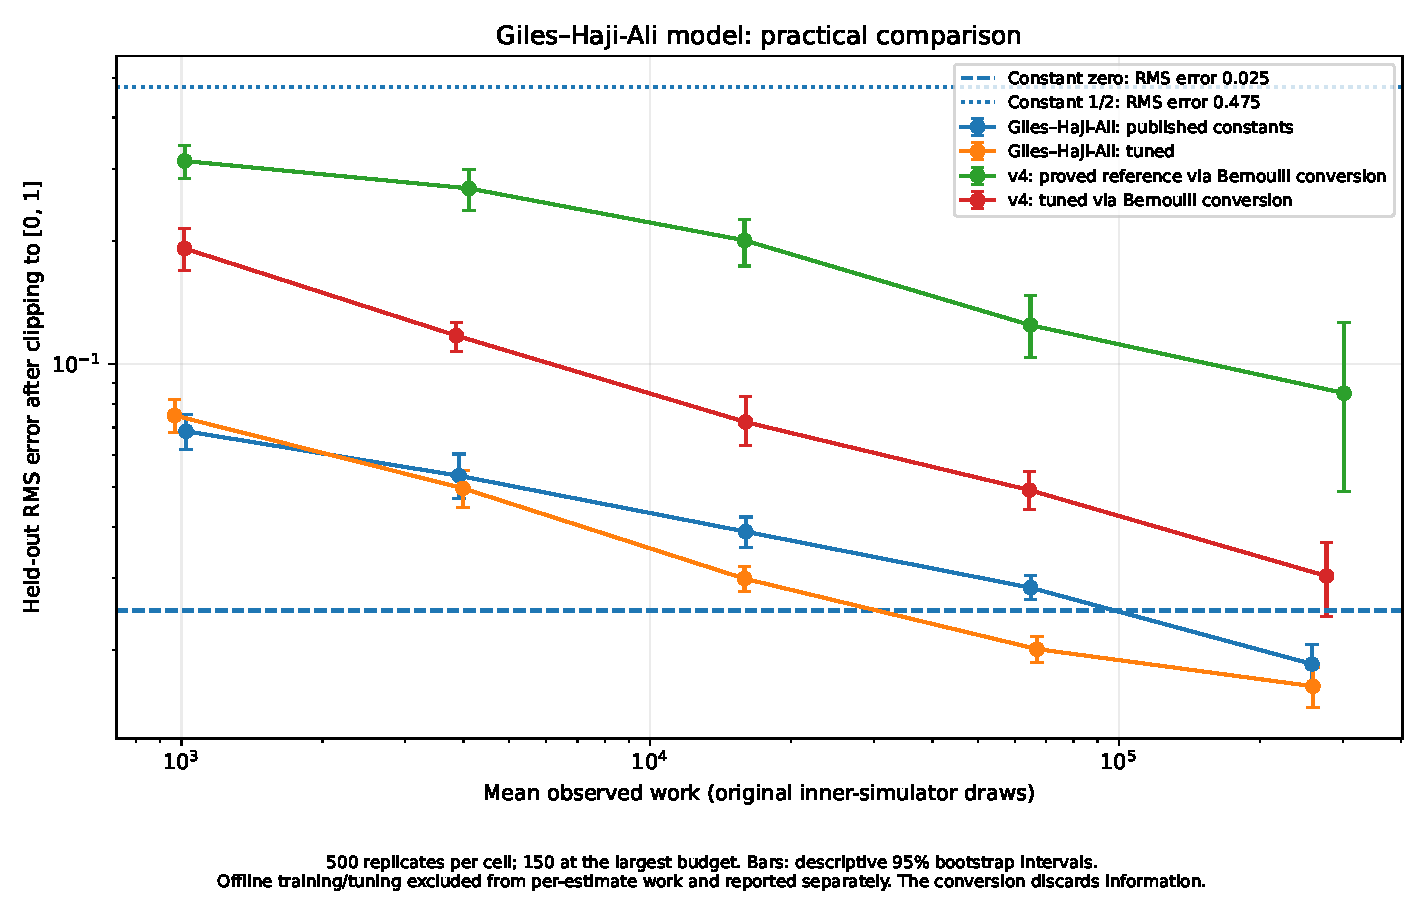
\includegraphics[width=\textwidth]{benchmark_rmse.pdf}
\caption{Numerical evidence only. Work is the measured mean number of original inner draws. All plotted estimates are clipped. Error bars are descriptive percentile-bootstrap intervals, not certified heavy-tail confidence intervals. Offline training/tuning and the information-loss caveat are described in the text.}
\end{figure}

At approximately $65{,}000$ observations, tuned GHA has RMS error $0.02012$, the tuned converted-v4 variant $0.04922$, and the proved converted-v4 reference $0.12443$. Thus tuning improves v4 materially but does not make it competitive here. At the largest budget the two nontrivial GHA multilevel implementations still win. The v4 reference's largest-budget mean work is noisy: about $302{,}035$ with standard error about $17{,}613$, rather than its nominal $262{,}144$. Expected-budget guarantees do not impose a hard limit on each run, and the sample mean itself is uncertain.

The constant-zero estimate has RMS error $0.025$ on this particular model. Most small-budget methods fail even that benchmark. The constant-$1/2$ estimate has RMS error $0.475$. Before clipping, the v4 reference has RMS errors $0.85245$ and $0.48224$ at the two smallest budgets, both worse than constant $1/2$. After clipping, its errors fall to $0.31331$ and $0.26849$. Clipping improves squared error but generally changes bias; these are not unbiased output claims.

Tuning is not guaranteed to help out of sample: at the smallest budget, tuned GHA has error $0.07487$, worse than the reference's $0.06851$, with overlapping descriptive intervals. We do not fit convergence exponents from these five budgets or use Monte Carlo results as evidence for any theorem. The conversion, fitted allocations, small replication count in the extension, and omitted offline costs prevent a universal practical-superiority conclusion. The actual observed comparison favors GHA.

\section{Verification record and unresolved work}
\status{Diagnostics and explicit completion limits}
The deterministic/numerical diagnostics executed in this phase comprise:
\begin{itemize}
\item 24 atomic-law constrained optimizations checked against Proposition~\ref{prop:optimizer}; largest objective discrepancy $2.85\times10^{-12}$.
\item 20 power-integral quadrature comparisons checking the analytic envelopes in Lemma~\ref{lem:integrals}.
\item 270 common-prefix agreement checks with the v4 classifier and 300 shifted-prefix checks against direct decisions on the same fixed tapes.
\item Direct evaluation of the counterexample's KL and Le Cam constants; the resulting lower coefficient is approximately $0.010697>1/100$.
\end{itemize}
These are finite diagnostics. They are not formal certificates of universal inequalities, independent expert reviews, or substitutes for the proofs. The benchmark has 8,000 initial and 600 extension held-out full-estimator runs; the raw outputs and costs are included. Bootstrap intervals use 3,000 resamples per cell and are descriptive only.

\textbf{Task 1 completion limit.} The conjectured heuristic has been disproved, a complete localized power-margin range has been proved, and a general lower modulus and upper bracket are supplied. The arbitrary-law matching upper bound, the regimes $\alpha\ge2$, and a distribution-blind localized upper algorithm are not settled here.

\textbf{Task 2 completion limit.} A targeted four-area comparison was carried out with primary-source citations and recorded inspection depth. Some neighboring papers remain abstract-only or inaccessible in full text. No priority certification follows.

\textbf{Task 3 completion limit.} The specified GHA model and published adaptive/coupling components were implemented, tuned independently, and tested. The v4 proof is retained only through a model-specific Bernoulli conversion. A direct real-valued adaptation of v4 and a comprehensive equal-total-training-cost study were not performed.

\textbf{Optional tasks.} No hard-cap theorem or arbitrary-law equality $\inf VW=I_\mu^2/16$ is claimed. Those were not pursued ahead of the unresolved main task.

\begin{thebibliography}{20}
\bibitem{baseline} A Distributional Minimax Law for Adaptive Threshold Estimation. Version 4, 26 October 2026. User-provided baseline PDF and source package; retained unchanged.
\bibitem{lv} J. C. H. Lee and P. Valiant. Uncertainty about Uncertainty: Optimal Adaptive Algorithms for Estimating Mixtures of Unknown Coins. SODA 2021; arXiv:1904.09228v3. \url{https://arxiv.org/html/1904.09228v3}. In particular Theorems 1--5, Lemmas 17--18, Corollary 19, and Section 7.
\bibitem{gha} M. B. Giles and A.-L. Haji-Ali. Multilevel nested simulation for efficient risk estimation. SIAM/ASA Journal on Uncertainty Quantification, 7(2):497--525, 2019. DOI:10.1137/18M1173186. \url{https://arxiv.org/pdf/1802.05016v2}. Algorithm 1 and equations (3.2)--(3.6).
\bibitem{chen} Z. Chen, M. Naslidnyk, and F.-X. Briol. Nested Expectations with Kernel Quadrature. ICML, PMLR 267, 2025. \url{https://arxiv.org/html/2502.18284v2}. Problem statement and Section 6 inspected.
\bibitem{wang} W. Wang, Y. Wang, and X. Zhang. Smooth Nested Simulation: Bridging Cubic and Square Root Convergence Rates in High Dimensions. Management Science, 2024. DOI:10.1287/mnsc.2022.00204; arXiv:2201.02958. Primary abstract/indexed material only in this audit; full theorem comparison not completed.
\bibitem{brennan} J. Brennan, R. K. Vinayak, and K. Jamieson. Estimating the Number and Effect Sizes of Non-null Hypotheses. arXiv:2002.07297, 2020. \url{https://arxiv.org/abs/2002.07297}. Section 1.1 and Theorem 2.1 inspected.
\bibitem{gotovos} A. Gotovos, N. Casati, G. Hitz, and A. Krause. Active Learning for Level Set Estimation. IJCAI, 2013, pp. 1344--1350. \url{https://www.ijcai.org/Proceedings/13/Papers/202.pdf}. Section 2 inspected.
\bibitem{hanneke} S. Hanneke and L. Yang. Minimax Analysis of Active Learning. arXiv:1410.0996, 2014. \url{https://arxiv.org/abs/1410.0996}. Primary abstract checked; full theorem comparison not completed.
\bibitem{aziz} M. Aziz, J. Anderton, E. Kaufmann, and J. Aslam. Pure Exploration in Infinitely-Armed Bandit Models with Fixed-Confidence. ALT 2018. \url{https://research.cs.cornell.edu/conferences/alt2018/A/aziz18Paper.pdf}. Sections 2.2 and 3 inspected.
\bibitem{pilliat} E. Pilliat. Adaptive Algorithms for Infinitely Many-Armed Bandits: A Unified Framework. arXiv:2510.27319, 2025. \url{https://arxiv.org/abs/2510.27319}. Primary abstract checked; full theorem comparison not completed.
\bibitem{mendo} L. Mendo. Asymptotically Optimum Estimation of a Probability in Inverse Binomial Sampling under General Loss Functions. Author preprint, 25 April 2012. \url{https://oa.upm.es/10749/1/asympt-opt16completo.pdf}. Introduction and equation (1), explicitly attributing the inverse-count estimator to J. B. S. Haldane (1945).
\bibitem{mendoh} L. Mendo and J. M. Hernando. Improved Sequential Stopping Rule for Monte Carlo Simulation. IEEE Transactions on Communications, 56(11):1761--1764, 2008. \url{https://arxiv.org/abs/0809.4047}. Primary abstract checked; full proof comparison not completed.
\bibitem{ibs} B. van Opheusden, L. Acerbi, and W. J. Ma. Unbiased and Efficient Log-Likelihood Estimation with Inverse Binomial Sampling. arXiv:2001.03985, 2020. \url{https://arxiv.org/abs/2001.03985}. Primary abstract checked; PMC full-text access was blocked during this audit.
\bibitem{vihola} M. Vihola. Unbiased Estimators and Multilevel Monte Carlo. arXiv:1512.01022v4. \url{https://arxiv.org/html/1512.01022v4}. Established randomization and variance--cost allocation; no novelty claim for these ingredients.
\bibitem{medin} S. C. Medin, J. Murray-Bruce, D. Casta\~n\'{o}n, and V. K. Goyal. Beyond Binomial and Negative Binomial: Adaptation in Bernoulli Parameter Estimation. arXiv:1809.08801v2, 2019. \url{https://arxiv.org/html/1809.08801v2}. Sections I and III and conclusion inspected.
\end{thebibliography}
\end{document}
